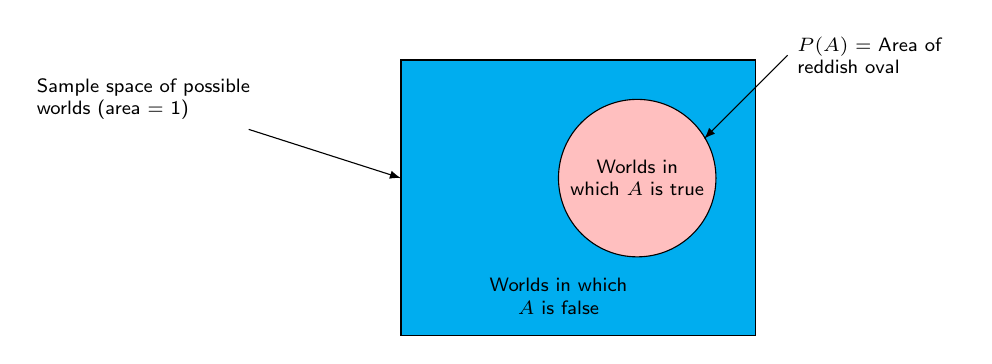
\begin{tikzpicture}[scale=0.5, font=\sffamily\scriptsize]


\draw[fill=cyan]  (-6,6) rectangle (3,-1);
\draw[fill=pink]  (0,3) ellipse (2 and 2) node [text width=2cm, text centered] {Worlds in which $A$ is true};

\node [text width=3cm, anchor=east] (t1) at (-9,5) {Sample space of possible worlds (area = 1)};

\coordinate (t2) at (-6,3);
\draw[-latex] (t1) -- (t2);
\node [text width=2cm, text centered] at (-2,0) {Worlds in which $A$ is false};
\draw[latex-]  (1.7,4) -- ++(45:3) node[anchor=west, text width=2cm] {$P(A)$ = Area of
reddish oval};
\end{tikzpicture}